\documentclass[10pt]{article}
\usepackage[T1]{fontenc}
\usepackage{lmodern,amsmath,amssymb,graphicx,hyperref,array}
\usepackage[margin=0.75in]{geometry}
\setlength{\parindent}{0pt}\setlength{\parskip}{6pt}
\begin{document}
\begin{center}
{\Large Pole-chart leading factors and actual anchor degree budget}\\[4pt]
14 November 2026; source \texttt{43b457291f5b99ae1c23c4057b34ad07bdb07b41}
\end{center}
\textbf{Component results.} The same completed orientation family has
explicit polynomial leading factors at its retained negative-pole charts,
with $2^u$ labels. Its actual diagonal degree also bounds the last retained
anchor multiplicity by a Fibonacci factor. The pinned shared gate audits
59 declarations with zero extra trusted axioms. Import-inclusive fresh
replay now exits 0 for OrientationCompletion, with imports included.
All records are unsigned [pcc:unverified].

\textbf{Actual chart, every coefficient.} Let $L=2^a$, $i<u\le a$,
$t=-2^i$, $\alpha=2^{a+1}$, and
\[
 M_{xy}=\{j<u:\operatorname{bit}_j(x)=\operatorname{bit}_j(y)\},\quad
 G_i=m_i-\sum_{j<u}(j-i)_+m_j.
\]
Use the original actual completed polynomial $W_{xy}(T)$ on actual ports
$x,y<2^a$, and equal-bit-$i$ crossings. Let $P_{xy}(Z)=W_{xy}(t+\alpha Z)$,
$J_{xy}=[Z]P_{xy}$, $c=J_{00}\ne0$, and
$w=v_2(c)=a+1-i+G_i$. No favorable scalar is supplied. Multiplicities are natural numbers; the
matrix leading-factor statements additionally require $m_j>0$ for every
$j<u$.
The finite rest product and actual anchor slopes construct a polynomial
$U_{xy}$ such that
\[
 P_{xy}=J_{xy}Z U_{xy},\qquad U_{xy}(0)=1,\qquad
 v_2([Z^n]U_{xy})\ge n
\]
with zero coefficients admitted. The full chart has content at least $w$,
so $J_{xy}/c$ is integral. Therefore
\[
 v_2([Z^{n+1}](P_{xy}/c))\ge n,\qquad
 P_{xy}/c\equiv (J_{xy}/c)Z\pmod 2
\]
coefficientwise. This is a universal symbolic statement at these specified
negative poles, not a sample of coefficients [pcc:unverified].

\textbf{Constructed matrix lift.} Zero entries outside the crossings.
The parent's actual first-jet factors $A,B$ satisfy $R-AB\equiv0\pmod2$,
$R_{xy}=J_{xy}/c$. Set $\widetilde A=C(A)$ and
$\widetilde B=C(B)Z$, with the same $2^u$ labels. Then
\[
 P/c-\widetilde A\widetilde B\equiv0\pmod2.
\]
Both factors are integral. Scaling the left by $C(c)$ gives row content
$w$ and actual residual content $w+1$; the scaled left is integral if
$w\ge0$. This covers the lowest precision layer of the whole polynomial
chart, not arbitrary precision or all active source nodes [pcc:unverified].

\newpage
\begin{center}{\Large A necessary budget for the actual polynomial}\end{center}
This page uses $n=u+1$ retained levels, with terminal level $u$; this is an
index convention, not an extra retained level in the chart theorem.
Construct the actual list $(m_0,\ldots,m_u)$ from the finite range. The
Lean bridge derives the abstract recurrence from the actual inequalities
$G_i\ge0$ for every $i<u+1$. A caller does not supply a feasible list.
For a list $\ell=(m_0,\ldots,m_{n-1})$, its weighted suffix penalty is
\[
 \operatorname{penalty}(\ell)=\sum_{j<n}(j+1)m_j.
\]
Prepending a multiplicity $m\ge P$ to an existing suffix of mass $S$ and
penalty $P$ gives
\[
 S'=m+S\ge P+S,\qquad P'=m+P+S\ge2P+S.
\]
Starting from the actual terminal multiplicity $r=m_u$, the initial suffix
has $S=P=r$. Fibonacci induction gives
\[
 F_{2u+1}m_u\le\sum_{j<u+1}m_j,\qquad
 F_{2u+2}m_u\le\operatorname{penalty}(m_0,\ldots,m_u).
\]
These are necessary inequalities for this explicit schedule, not a
lower bound for arbitrary completion polynomials [pcc:unverified].

\textbf{Exact degree, not reversal of an upper bound.}
For a finite source set $S\subset\mathbb Q$ with $0\in S$, the actual
normalizer is nonzero and the diagonal base has degree $|S|-1$.
Every selected factor is nonzero of degree one. At $x=y$ the actual mask
selects all retained anchors. Degrees add over $\mathbb Q$, giving
\[
 \deg W_{xx}=|S|-1+\sum_{j<u+1}m_j.
\]
For the actual signed grid $|S|=2L$, an actual diagonal cap
\[
 \deg W_{xx}\le 2L-1+KL
 \quad\Longrightarrow\quad F_{2u+1}m_u\le KL.
\]
The previous upper-degree estimate alone would not justify this direction.
Nonzero selected factors and the actual normalizer are derived in the proof
[pcc:unverified].

\textbf{Proof map.} Full statements, source bindings and all 54 new unsigned
claim ids are in \path{../evidence/claim-pins.json}. Central declarations:
\begin{center}\small
\begin{tabular}{p{0.59\linewidth}p{0.29\linewidth}}
\texttt{actual\_completed\_chart\_unit} & PCC-20261114-4e9529\\
\texttt{actual\_normalized\_coefficient\_weight} & PCC-20261114-0be10e\\
\texttt{actual\_chart\_leading\_factorization} & PCC-20261114-141d98\\
\texttt{actual\_weighted\_chart\_leading\_factorization} & PCC-20261114-dc6a99\\
\texttt{actual\_schedule\_feasible} & PCC-20261114-d08950\\
\texttt{completed\_diagonal\_degree} & PCC-20261114-b4a0e7\\
\texttt{actual\_terminal\_polynomial\_budget} & PCC-20261114-2d4b00
\end{tabular}
\end{center}
All are unsigned/default not covered; the full Lean statement governs each
claim's hypotheses [pcc:unverified].

\newpage
\begin{center}{\Large Mode cost: the comparison that must still be made}\end{center}
The pinned primary proof D.4.3--D.4.7 has $D_i=L/2^i$, at most $3M/L$
packets, precision $p_t=O(MD_i/u)$, and at most $6M/D_i$ modes per weight.
Its weighted tuple bound is $\exp(O(\sqrt{Mp_t/D_i}))$, yielding
$\exp(O(M/\sqrt u))$. These are the reviewed primary proof's formulas,
not a new measured or independently formalized runtime result
[pcc:unverified].

For the separate actual first-jet moment construction, every residue class
$r\bmod2^u$ and every retained moment $b$ is charged. The corresponding
\emph{declared} per-weight inventories and bounds are:
\begin{center}
\begin{tabular}{lcc}
 & Original primary profile & Residue moment profile\\\hline
labels per packet per moment & $2^{i+1}$ & $2^u$\\
public row weight & $b+1$ & $w+b$\\
packet-count upper budget & $6M/D_i$ & $(3M/L)2^u$
\end{tabular}
\end{center}
The ratio of those declared upper budgets is $2^{u-i-1}$. It is not an
observed count ratio or a lower bound for the number of independent nonzero
modes. Higher coefficient valuations, zero coefficients or a different basis
could change the relevant inventory. A smaller symbolic factor count than
row refinement does not settle the original comparison [pcc:unverified].

\begin{center}
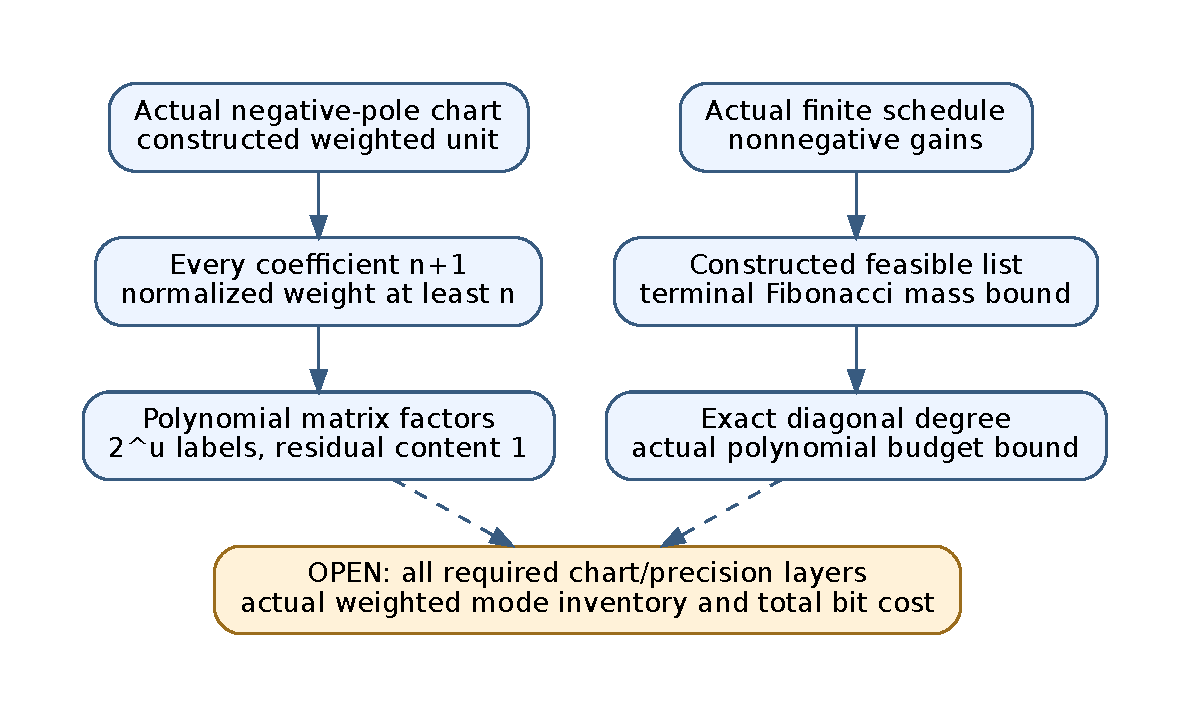
\includegraphics[width=0.95\linewidth,height=3.2in,keepaspectratio]{dependencies.pdf}
\end{center}
\textbf{Next discriminating obligation.} Construct and charge the actual
weighted mode inventory, including coefficient construction and target/source
locality. Combine it with the exact degree cap, required precision and
recovery loss. The negative-pole lowest-layer statement cannot be substituted
for all required charts or higher precision. A full prime-field ECDLP proof
also needs the actual relation map, public finder, field/scalar extraction,
retry bounds and complete expected bit cost.

\newpage
\begin{center}{\Large Evidence, scope and reproducibility}\end{center}
\textbf{Checks.} The source contains 57 authored statements: 33 pole-chart
and 24 budget statements. Three are copied historical budget lemmas; 54 are
new source-bound declarations. The shared gate audits 59 declarations,
including these generated declarations:
\begin{center}\texttt{AnchorBudget.Feasible.brecOn}\\
\texttt{LocalCharts.localBase.eq\_1}\end{center}
All three new tracked modules were built and audited. Local build and gate
exit 0. Import-inclusive fresh replay exits 0, with imports included:
\begin{center}\texttt{leanchecker --fresh --verbose OrientationCompletion}\end{center}
Exact stdout is 45 bytes; raw log and exit status are retained [pcc:unverified].

\textbf{Pinned dependencies.} Lean 4.35.0, with:
\begin{center}\small
CryptoLean \texttt{148f5dc389b341401e06d76abe7783c4ccf42f2e}\\
Mathlib \texttt{cfc55fc58714a59dc06e6e79edc6d1d95140d3c2}
\end{center}
Exact source, manifest, gate, audit and trust hashes are in
\path{../evidence/source-freeze.json}. Gate data is PCC-20261114-67cb41.
Local draft records 623aab, 92e0dc, b83c13, a4c256 and 73e030 preserve
intermediate status. The axioms shown are only \texttt{propext},
\texttt{Classical.choice} and \texttt{Quot.sound} [pcc:unverified].

\textbf{Failures retained.} Chart 006 rewrite/visibility and 008 helper
normalization failures; budget 001 path failure, 002 recurrence/normalization,
003 zero-add, 004 unused-tactic warnings and 007 factor-unfolding failure.
All raw source/log/exit versions remain under the moment evidence directory.
Rejected drafts' sorryAx diagnostics are failures, not accepted proof inputs.
No warnings were suppressed; frozen parent source and report checkpoints
were not changed. There was no native cryptographic, timing, scaling or
paid/cloud experiment in this round.

\textbf{Sources checked.} KB unavailable: not loaded, wrapper has no
executable; the journal records bounded GitHub fallback queries. Read the
original AnchorBudget, actual OrientationAnchor/Leading/Jet and
LocalCharts/Integral sources, pinned Mathlib list/degree/coefficient APIs,
and the primary D.4.3--D.4.7 with source-triage, contraction-cost and
contraction-precision reviews under
\begin{center}\small\path{research/prime_one_shot_20261029/continuation/tensor-review/}\end{center}
Primary PDF SHA256, split for legibility:
\texttt{5b1612dc2eebb2cad5b4cbe62d1fed2982}\\
\texttt{f01ab1908c26f70010a651487e8123}.
Standard inverse moments, Fibonacci induction and polynomial degree laws
are reused; there is no priority or fastest-method assertion.

\textbf{Graph/evidence policy.} This is a symbolic proof-component report,
so the graphic is a dependency diagram, not an empirical plot. The literal
parent ring-scaling certificate IDC1h57849461da3c8854 remains limited to its
fixed 32+16 points and is not a certificate of these parameterized valuations,
Fibonacci bounds or runtime. No new measurement supports changes to the
IC scoreboard/timeline/leaderboard or historical parent figures; these stay
unchanged. Editable DOT/SVG/PDF and this TeX/PDF are kept together.

\textbf{Integration.} PR4118's concurrent protected PCC ledger conflict
remains unresolved. Both histories and all claim/evidence bytes are
preserved. Auto-merge stays off pending a legitimate canonical-maintainer
reconciliation contract and actual-head gates. This integration dependency
is separate from the mathematical work.
\newpage
\begin{center}{\Large Separate local draft: terminal gain relative to $D$}\end{center}
\textbf{Status.} This appendix describes a separate five-statement local
Lean draft. It is \emph{outside} the frozen 57-statement source, 59-declaration
axiom audit and completed fresh replay. Exact source/log hashes are in
\begin{center}\small\path{../evidence/cost-relative-elaboration-001.json}\end{center} Data claim
PCC-20261114-9b0604. Local elaboration exits 0 without warnings and central
printed foundations are standard only [pcc:unverified].

\textbf{Finite scale inequality.} Let the terminal level be $2k$, with
$2k+1$ retained levels, all actual schedule inequalities nonnegative, and
$2k\le a$. Assume the actual diagonal polynomial obeys
\[
 \deg W_{xx}\le (2L-1)+KL,\qquad L=2^a.
\]
The already frozen actual polynomial budget implies
$F_{4k+1}m_{2k}\le KL$. Standard Fibonacci addition gives
\[
 F_{n+4}=2F_n+3F_{n+1}\ge5F_n,
 \qquad F_{4k+1}\ge5^k.
\]
The exact power split and the actual budget therefore give
\[
 L=4^k2^{a-2k},\qquad 5^km_{2k}\le K4^k2^{a-2k}.
\]
All denominators below are positive; rational division yields
\[
 \boxed{\frac{m_{2k}}{D_{2k}}\le K(4/5)^k},\qquad D_{2k}=2^{a-2k}.
\]
The primary retained-node application also keeps its usual $2k+1\le a$
and other source hypotheses [pcc:unverified].

\textbf{Proof map.} All five declarations are in namespace
\texttt{OrientationBudgetScale}, file
\path{../evidence/cost-draft-002.lean.txt}:
\begin{itemize}
\item \texttt{fibonacci\_four\_growth};
\item \texttt{fibonacci\_geometric};
\item \texttt{actual\_terminal\_geometric};
\item \texttt{power\_split};
\item \texttt{actual\_terminal\_relative\_scale}.
\end{itemize}
This is a finite necessary bound on the terminal multiplicity under the
specified schedule and actual degree cap. It bounds the multiplicity
contribution, not the whole starting valuation $w$, which also contains
$a+1-2k$. It does not establish the actual nonzero-mode inventory, account
for possible coefficient sparsity/correlations, or prove an asymptotic
runtime or algorithm lower bound [pcc:unverified].

The failed first draft and raw compiler outputs remain archived. The repair
normalizes product associativity and removes over-general tactics without
changing hypotheses or suppressing a linter.

\newpage
\begin{center}{\Large Prior experiment audit: additive factor-base test}\end{center}
\textbf{Source-level finding.} The tracked constructor scans an arithmetic
progression but skips nonliftable $x$ values. It returns at the requested
size without enforcing constant gaps, then constructs the constraint from
the filtered coordinates. Its matching report already acknowledges this
caveat. This does not establish that the stated full falling-factorial
constraint was tested
[pcc:unverified].

The tracked $F_3(x_R,X_2,X_3)$ arm uses two base variables. Its pair-sum
control tests $R-P_k=P_i+P_j$, using three base points. Sage's fixed random
seed does not seed \texttt{secrets.randbelow}; arms draw separate scalar
targets. The $F_3$ branch counts coordinate membership without a signed
point equality check there. These are source observations, not a demonstrated
false witness or timing bias [pcc:unverified].

\begin{center}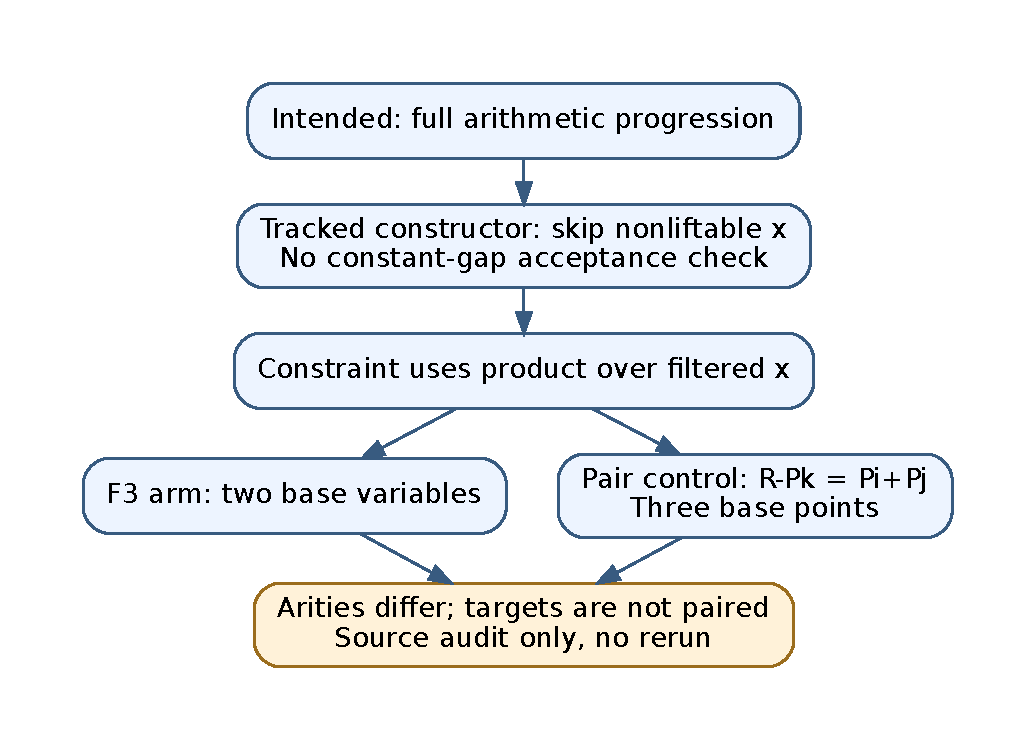
\includegraphics[width=0.86\linewidth,height=3.1in,keepaspectratio]{../prior-review/construction.pdf}\end{center}
\textbf{Evidence boundary.} Exact source/report snapshots, Git blobs and
hashes are in\begin{center}\small\path{../prior-review/source-review-001.json}\end{center} Literature data
claim PCC-20261114-6d5330. The historical report lacks raw-run/source-version
binding sufficient to identify the executed version uniquely. No old timing
is remeasured and no CPU-contention explanation is asserted. A genuine AP
can have step one; filtering, not that step value, is the issue
[pcc:unverified].

\textbf{Reason for a controlled retry.} Require actual base coordinates
with constant nonzero gaps and the intended polynomial identity before
timing; match decomposition arity and public target list, check signed
relations, charge construction and solver work, and retain all controls and
failures. No solver/timing campaign is launched here. This audit does not
close or certify the structured-base direction.

\newpage
\begin{center}{\Large Final replay status and preserved checkpoint}\end{center}
\textbf{Completed check.} Import-inclusive
\texttt{leanchecker --fresh --verbose OrientationCompletion} exits 0.
The exact 45-byte stdout is:
\begin{center}\texttt{replaying OrientationCompletion with --fresh}\end{center}
Raw log, exit and source/gate hashes are in
\path{../evidence/fresh-validation-001.json}; data PCC-20261114-5fe0c8.
These are unsigned replay observations, not a signed PCC verdict
[pcc:unverified].

\textbf{Exact scope.} The source remains
\begin{center}\small\texttt{43b457291f5b99ae1c23c4057b34ad07bdb07b41}\end{center}
It contains 57 authored statements, of which 54 are new and three are copied
historical budget lemmas. The shared gate audits 59 declarations, including
the two generated declarations listed on page four, with zero extra trusted
axioms. No mathematical source changed between source freeze, gate and fresh
replay [pcc:unverified].

\textbf{Preservation.} All 74 original checkpoint artifact hashes still
match, including the original pending report, study README, protocol and
dated report. This final report is a versioned addition; the old pending
snapshot and its claim are historical, not rewritten. Earlier successor and
moment checkpoint hashes also match. Parent source, claims, ledger prefixes,
raw logs and artifact-storage conventions are preserved [pcc:unverified].

\textbf{Separate local material.} The five-statement finite relative-scale
draft remains outside this source/gate/fresh scope. The additive-FB review
is pinned source analysis; no historical run is remeasured or newly attested.
No native cryptographic, solver, timing or cloud campaign ran in this round.

\textbf{Next proof obligation.} Extend graded content to arbitrary retained
source-node charts, including positive anchors where a correction value can
vanish. Derive coefficient bounds directly rather than divide by an assumed
unit. Then construct required matrix/precision layers and charge the actual
nonzero modes, entry/bit/recovery/recursion costs and public prime-field
finder/extraction/retry procedure.

The protected concurrent ledger reconciliation remains a separate integration
dependency. Auto-merge is off; no protected history, claim, signature, trust
entry or required gate is changed by this final check.

\end{document}
